\PassOptionsToPackage{dvipsnames}{xcolor}
\documentclass[11pt,letterpaper]{article}
\usepackage{mathalpha}
\usepackage{algorithm}
\usepackage{algorithmicx}
\usepackage{algpseudocode}
\usepackage{graphicx}
\usepackage{subcaption}
\usepackage{booktabs}
\usepackage{float}
\usepackage{bm}
\usepackage{mathtools}
\usepackage{mathrsfs}
\usepackage{nicefrac}
\usepackage{listings}
\usepackage{dsfont}
\usepackage{fdsymbol}
\usepackage{array}
\usepackage{multicol}
\usepackage{multirow}
\usepackage{url}
\usepackage{fancyhdr}
\usepackage{rotating}
\usepackage{tikz}
\usetikzlibrary{shapes,arrows,positioning,calc}
\usepackage{pgfplots}
\pgfplotsset{compat=1.16}
\usepackage[a4paper, margin=1in]{geometry}
\usepackage{colortbl}
\usepackage{xcolor}
\usepackage{enumitem}
\setlist[itemize]{leftmargin=*,noitemsep,topsep=3pt}
\setlist[enumerate]{leftmargin=*,noitemsep,topsep=3pt}

% Citation and bibliography setup
\usepackage[comma,numbers,compress]{natbib}
\bibliographystyle{plainnat}

% Caption setup
\usepackage[font=small,labelfont=bf]{caption}

% Color definitions
\definecolor{lightblue}{rgb}{0.22,0.45,0.70}
\definecolor{YaleBlue}{rgb}{0.06,0.30,0.56}
\definecolor{memstblue}{RGB}{41, 98, 255}

% Hyperref setup
\usepackage{hyperref}
\hypersetup{
    colorlinks = true,
    citecolor = {YaleBlue},
    linkcolor = {YaleBlue},
    urlcolor  = {YaleBlue}
}
\usepackage{hypcap}

% Cleveref must be loaded AFTER hyperref
\usepackage[capitalise]{cleveref}

% Custom commands
\newcommand{\memst}{\textsc{MemSt}}
\newcommand{\memzero}{\textsc{Mem0}}
\newcommand{\Fone}{\textsc{F1}}
\newcommand{\Bone}{\textsc{BLEU-1}}

\title{\centering \textbf{\memst}: Adaptive Semantic Memory for Production AI Agents}
\author{\centering Yifan Yang\\
\vspace{0.5em}
\hspace{0.6cm} \href{mailto:yfyang.86@hotmail.com}{\texttt{yfyang.86@hotmail.com}}}

\pagestyle{fancy}
\fancyhf{}
\fancyhead[C]{\textit{\fontsize{9}{11}\selectfont \memst: Adaptive Semantic Memory for Production AI Agents}}
\fancyfoot[C]{\thepage}
\addtolength{\headheight}{12pt}

\begin{document}

\maketitle

%==============================================================================
\begin{abstract}
\vspace{0.3cm}

Persistent memory remains a core limitation of large language model agents. While humans naturally recall facts, timelines, and relationships across long time horizons, most agent memory systems apply a single retrieval mechanism to every query, regardless of its structure. We introduce \memst, a semantic memory architecture that treats retrieval as a \textit{query-dependent optimization problem} rather than a uniform lookup operation.

The central insight behind \memst\ is that factual lookup, temporal reasoning, and relational traversal require different memory organizations. Instead of forcing all questions through one retrieval pipeline, \memst\ routes each query to a specialized strategy: Cascade filtering for direct factual retrieval, MultiHopKG for relational chains, TemporalKG for time-aware reasoning, and Hierarchical Summary for open-domain questions. A lightweight rule-based classifier selects among these strategies at inference time.

We evaluate \memst\ on the LOCOMO benchmark, using 1,540 answerable questions from 10 extended conversations after excluding 446 adversarial questions following prior work. \memst\ achieves \textbf{49.2\% F1}, improving over the strongest published managed-memory baseline by \textbf{41\%} and over standard retrieval-augmented generation by \textbf{118\%}. The gain does not come from routing alone. Even under fixed-strategy comparisons, \memst's architectural choices---tiered storage, token-budget-aware context assembly, and importance-guided retrieval---yield \textbf{46\% higher F1} than equivalent RAG configurations. The system remains efficient: hierarchical retrieval requires only 85 milliseconds median search latency, 3.3 times faster than comparable RAG pipelines, while end-to-end latency remains low.

Our analysis shows why adaptive retrieval matters. Multi-hop questions routed through single-hop retrieval lose 65\% of their attainable performance, and temporal questions answered through generic retrieval lose much of the benefit of explicit timeline structure. These findings suggest that next-generation agent memory should be adaptive not only in what it stores, but also in how it is accessed.

\vspace{2mm}
\noindent\textbf{Code}: \href{https://github.com/yfyang86/memst}{https://github.com/yfyang86/memst}
\end{abstract}

%==============================================================================
\section{Introduction}
\label{sec:intro}

Human memory is selective rather than uniform. When asked ``When did Alice move to San Francisco?'', we retrieve temporal information; when asked ``Who is Alice's manager's spouse?'', we follow a chain of relationships; when asked ``Tell me about Alice'', we synthesize episodes into a coherent summary. Cognitive science has long suggested that memory is not a single mechanism, but a family of systems adapted to different forms of recall \citep{tulving2002episodic, atkinson1968human}. What matters is not only what is stored, but how it is accessed.

Contemporary AI agents lack this flexibility. Large language models operate within finite context windows, and even very large windows do not solve the broader problem of persistent memory across repeated interactions \citep{bulatov2022recurrent, liu2023think}. External memory systems address this limitation by storing information beyond the prompt, but most still apply the same retrieval strategy to every query. In practice, a direct factual lookup, a temporal comparison, and a multi-hop relational question often receive the same treatment, typically some variant of vector search or flat hybrid retrieval.

This uniformity is costly. Consider a question such as ``Why did Alice leave her previous company?'' A flat retrieval system may surface passages mentioning Alice, the company, or departure events, yet still fail to connect them with a separate statement such as ``Alice disliked the remote work policy.'' The facts may all be present, but the retrieval structure is mismatched to the question. As a result, the system retrieves evidence without recovering the relation that makes the answer possible.

\subsection{The Query-Adaptivity Hypothesis}

We hypothesize that memory retrieval should be \textit{query-dependent}: the best strategy for locating a specific fact is not the best strategy for traversing relationships, constructing a timeline, or summarizing broad context. If this hypothesis is correct, an effective agent memory system should not merely store more data or retrieve more text. It should select retrieval structures that match the informational demands of the query.

Realizing this idea requires more than adding a router on top of an existing memory stack. It requires specialized retrieval strategies whose inductive biases align with different question types, a routing mechanism accurate enough to exploit those differences, and a systems design efficient enough that adaptivity does not cancel its own gains through overhead. Query-adaptive memory is therefore useful only if it is both algorithmically justified and operationally practical.

\subsection{Contributions}

This paper introduces \memst, a semantic memory architecture built around query-adaptive retrieval. The system is designed from the premise that persistent memory should be treated as an active computational substrate rather than a passive store of embedded text. Its contributions span retrieval design, storage architecture, and empirical analysis.

\textbf{Specialized retrieval strategies.} We develop four retrieval strategies tailored to distinct query types. Cascade retrieval applies progressive filtering for high-precision factual lookup. MultiHopKG constructs entity-relation graphs for compositional traversal. TemporalKG extracts and normalizes time expressions for chronological reasoning. Hierarchical Summary organizes memory at multiple granularities for open-domain questions.

\textbf{Lightweight query classification.} We implement a rule-based classifier achieving 80\% accuracy on LOCOMO question types. Although simple, it delivers a substantial gain in aggregate performance: adaptive routing improves over the best fixed strategy by 7.5 F1 points. Temporal questions are easiest to classify (91.7\% accuracy), while open-domain questions are the most ambiguous (77.1\%).

\textbf{Production-oriented memory infrastructure.} \memst\ combines content-addressable storage with Blake3 hashing, write-ahead logging, and a four-tier memory hierarchy. This design supports deduplication, integrity verification, bounded prompt construction, and lifecycle management while remaining efficient in practice.

\textbf{Comprehensive evaluation.} On LOCOMO, using 1,540 evaluated questions from 1,986 total after excluding 446 adversarial questions, \memst\ reaches 49.2\% F1. This substantially exceeds standard RAG and published memory baselines. Under matched fixed-strategy settings, \memst\ also outperforms equivalent RAG configurations, showing that the gains arise not only from routing but from the underlying organization of memory itself.

%==============================================================================
\section{Background and Related Work}
\label{sec:background}

The problem of long-horizon memory in LLM agents has attracted growing attention because context-window scaling alone has not solved the practical demands of persistent interaction. Existing approaches can be grouped into several broad families, each capturing an important insight while leaving a complementary gap.

Architectural approaches attempt to internalize longer memory directly within the model. Systems such as Recurrent Memory Transformer \citep{bulatov2022recurrent} and related long-context mechanisms extend the effective receptive field through recurrence, compression, or sparse attention. These methods are elegant because they preserve end-to-end differentiability and avoid explicit external storage. Yet they remain bounded by model capacity, context management overhead, and inference cost. In practice, they improve how much a model can \emph{hold} at once, but not necessarily how selectively it can \emph{retrieve} from months of accumulated interaction.

A second line of work externalizes memory into vector databases and retrieval systems. Platforms such as Chroma, Pinecone, and Milvus provide scalable semantic search and have become the default memory substrate for many agent frameworks. Their appeal lies in simplicity: embeddings are easy to produce, approximate nearest-neighbor search is efficient, and the interface is general-purpose. At the same time, this generality is also their main limitation. A flat vector store treats all memories as interchangeable retrieval units, even though conversational memory is structurally heterogeneous. A user preference, a temporal sequence of events, and a social relationship graph are not merely different embeddings of the same object; they are different informational structures that often require different access patterns.

Hierarchical memory systems take a more cognitively and systems-inspired view. MemGPT \citep{packer2023memgpt} proposed operating-system-style paging across memory tiers, while MemoryBank \citep{zhong2024memorybank} introduced reinforcement and forgetting mechanisms. These systems correctly emphasize that memory is not just about retrieval, but also about allocation, compression, and lifecycle management. Their central intuition is that durable intelligence requires structure over time. However, they largely assume that once memory is organized hierarchically, retrieval itself can remain uniform. Our results suggest that this assumption is incomplete: hierarchy helps, but hierarchy alone does not resolve the mismatch between question type and retrieval strategy.

Knowledge-graph-based systems, including Zep \citep{rasmussen2025zep} and A-MEM \citep{xu2025mem}, address a different weakness of flat retrieval by introducing explicit relational structure. These systems are particularly effective when answers depend on compositional reasoning across entities, relations, and events. Their contribution is to show that some memories are better represented as graphs than as text chunks. At the same time, generic graph memory can become overly rigid if used indiscriminately. Not every question benefits from traversal; in many cases, direct lexical retrieval or hierarchical summarization is both cheaper and more accurate.

Managed memory services such as \memzero~\citep{chhikara2025mem0} demonstrate that persistent memory can be exposed as a practical API and can materially improve downstream agent quality. Their importance is infrastructural as much as empirical: they show that memory is becoming a first-class systems component. However, managed services typically optimize for ease of integration and stable abstractions, which can limit visibility into retrieval behavior, provenance, and memory evolution.

Taken together, the literature reveals a consistent pattern. Most prior systems optimize \emph{one axis} of memory design at a time: larger internal context, better vector retrieval, hierarchical organization, or explicit graph structure. \memst\ is motivated by the observation that real conversational recall draws on all of these ideas, but not in the same way for every question. The key intuition behind our approach is therefore simple: \emph{memory should be adaptive not only in what it stores, but in how it is accessed}. A factual question benefits from precision-oriented filtering; a relational question benefits from graph traversal; a temporal question benefits from normalized timelines; and an open-ended question benefits from coarse-to-fine summarization.

Our contribution is not to claim novelty for content-addressable storage, hierarchical memory, or graph extraction in isolation. Rather, the innovation of \memst\ lies in showing that these components become substantially more effective when coupled through query-adaptive routing. In this sense, \memst\ advances the literature from static memory architectures to \emph{retrieval-conditioned memory systems}: systems whose organization is not merely persistent, but dynamically aligned with the informational form of the question being asked.

%==============================================================================
\section{The \memst~Architecture}
\label{sec:architecture}

At a high level, \memst\ separates the memory problem into three questions: how information should be stored, how it should be organized over time, and how it should be retrieved for a given query. Much prior work emphasizes only one of these dimensions. Our design treats them as inseparable. Storage determines what provenance and durability are available; organization determines what remains salient, compressed, or archived; and retrieval determines whether the appropriate structure is exposed at inference time. The architecture is therefore not a collection of independent modules, but a coordinated memory pipeline in which each component reinforces the value of the others.

\memst\ comprises three interconnected subsystems: (1) a \textbf{versioned storage layer} for content-addressable persistence; (2) \textbf{specialized retrieval strategies} optimized for distinct query types; and (3) a \textbf{rule-based classifier} that routes queries to appropriate strategies.

\subsection{Versioned Storage Layer}
\label{sec:storage}

Our storage design draws inspiration from Git's content-addressable model, although the analogy is partial rather than literal.

\textbf{Content-addressable objects.} We implement three object types using Blake3 addressing. \emph{Blobs} store message content and embeddings, addressed by $\text{Blake3}(\text{content})$. \emph{Trees} map conversation identifiers to blob hashes, enabling hierarchical organization. \emph{Commits} capture memory snapshots with parent references, timestamps, and metadata, forming an immutable audit trail.

This design naturally provides deduplication and integrity verification. Identical content is stored once regardless of repetition, reducing storage by 12--18\% in our conversational workloads. More importantly, the commit structure preserves provenance: any memory state can be reconstructed from the commit graph, enabling debugging, rollback, and auditability in production settings.

\textbf{Write-ahead logging.} All mutations pass through a write-ahead log (WAL). Each operation is serialized with a checksum, durably persisted via \texttt{fsync}, then applied to in-memory state. Periodic checkpoints flush state to the object store. On recovery, the system replays WAL entries from the most recent checkpoint. This provides crash consistency without requiring a heavyweight database layer.

\textbf{Branching and isolation.} \memst\ supports worktrees: isolated working directories backed by a shared object store. This allows multiple agents or sessions to operate on distinct branches without copying the full memory substrate. Three-way merge for conflicting branches remains future work; at present, conflicts must be resolved manually or with application-specific logic.

Although we use Git-style terminology such as \emph{commit}, \emph{branch}, and \emph{checkout}, the semantics are adapted for agent memory. Commits represent session-level memory states rather than per-message history, balancing traceability against overhead.

\subsection{Four-Tier Memory Hierarchy}
\label{sec:hierarchy}

\memst\ organizes memory into four tiers reflecting access frequency, importance, and retrieval cost.

Working memory contains the active conversational context under a strict token budget (default 2,048 tokens). When the budget is exceeded, content is promoted or demoted based on recency and salience. Short-term memory retains recent facts under a time-to-live policy (default 7 days), while Long-term memory stores information deemed persistently important. Archival memory holds rarely accessed historical data in compressed form, potentially on slower storage, while preserving semantic indexing.

Promotion into Long-term memory is governed by an importance score:
\begin{equation}
I(m) = 0.4 \cdot \text{access\_freq}(m) + 0.3 \cdot \text{user\_rating}(m) + 0.3 \cdot \text{entity\_density}(m),
\end{equation}
where access frequency measures normalized retrieval count over a 30-day window, user rating captures explicit feedback when available, and entity density measures named entities per token. These weights were chosen by grid search on a validation subset of LOCOMO. Performance remains stable within approximately $\pm 1\%$ across nearby settings.

\textbf{Token-budget-aware context assembly.} A distinctive feature of \memst\ is that prompt construction is treated as a constrained optimization problem rather than a fixed top-\(k\) retrieval step:
\begin{align}
\text{maximize} \quad & \sum_{m \in S} R(m, q) \cdot I(m) \\
\text{subject to} \quad & \sum_{m \in S} \text{tokens}(m) \leq B_{\text{context}}, \quad |S| \leq 20.
\end{align}
Here \(R(m,q)\) denotes relevance and \(I(m)\) denotes memory importance. We use a greedy approximation that sorts candidates by \(R(m,q)\cdot I(m)\) and fills the budget until exhausted. On sampled subsets, this strategy performs within 2.8\% of an exact integer-linear-programming solution while reducing computation time by roughly two orders of magnitude.

\subsection{Hybrid Search Architecture}
\label{sec:hybrid}

\memst\ combines lexical and semantic retrieval signals through reciprocal rank fusion (RRF):
\begin{equation}
\text{RRF}(d)=\frac{w_{\text{BM25}}}{k+\text{rank}_{\text{BM25}}(d)}+\frac{w_{\text{vec}}}{k+\text{rank}_{\text{vec}}(d)},
\end{equation}
with \(k=20\) and category-specific weights. Single-hop questions favor BM25 because exact lexical matches are often decisive, whereas temporal and open-domain queries rely more heavily on semantic similarity.

Our native Rust BM25 implementation uses \(k_1 = 0.5\) and \(b = 0.75\), with the lower \(k_1\) reducing term-frequency saturation on short conversational turns. Dense retrieval uses HNSW approximate nearest-neighbor search with float16 vector storage, reducing memory use while maintaining fast lookup.

%==============================================================================
\section{Specialized Retrieval Strategies}
\label{sec:strategies}

The central architectural claim of \memst\ is that memory retrieval should not be uniform. Different queries induce different retrieval problems, and those differences justify different retrieval structures.

\subsection{Cascade Retrieval: Single-Hop Optimization}
\label{sec:cascade}

Single-hop questions demand precise factual lookup. A query such as ``What is Alice's job?'' typically has a localized answer and benefits from progressive filtering rather than graph traversal or broad summarization.

Cascade retrieval addresses this through three stages. First, BM25 selects 50 candidate memories from the full corpus, prioritizing recall. Second, vector similarity reranks the candidates down to the top 10, improving semantic precision. Third, a lightweight heuristic reranker scores the final candidates using token overlap, match position, and length normalization.

This staged design allocates expensive computation only where it is useful. Cascade achieves 55.2\% F1 on single-hop questions. Under a matched three-stage comparison, \memst-Cascade reaches 39.8\% overall F1 versus 27.3\% for RAG-Cascade, indicating that the gains arise not only from using a cascade pattern, but from the surrounding memory architecture.

\subsection{MultiHopKG: Relationship Traversal}
\label{sec:multihop}

Queries such as ``Who is Alice's manager's spouse?'' require composition across multiple facts. Flat retrieval often retrieves relevant fragments without connecting them. MultiHopKG addresses this by constructing a knowledge graph through entity-relation extraction and performing bounded traversal over the resulting structure.

For multi-hop questions, the system conducts breadth-first search up to two hops from the query entity. This supports retrieval over relational paths that are difficult to reconstruct from isolated text chunks. MultiHopKG achieves 52.8\% F1 on multi-hop questions, compared with 34.7\% overall F1 when forced to answer all question types uniformly. The gap is instructive: graph traversal is powerful when the query demands it, but it should not be applied indiscriminately.

\subsection{TemporalKG: Time-Aware Reasoning}
\label{sec:temporal}

Temporal questions require more than text retrieval. They depend on explicit normalization and ordering of events. A query such as ``When did Alice move to San Francisco?'' or ``Did Alice start before Bob's promotion?'' cannot be handled reliably if temporal expressions are treated as ordinary tokens.

TemporalKG extracts absolute dates, relative times, and implicit temporal references, then normalizes them against the conversation timeline. Events are organized into per-entity chronological sequences, enabling retrieval that respects temporal structure rather than surface similarity alone. TemporalKG achieves 54.0\% F1 on temporal questions, compared with 29.0\% overall F1 across all question types and 24.5\% for the RAG baseline on temporal questions.

\subsection{Hierarchical Summary: Open-Domain Context}
\label{sec:hierarchical}

Open-domain questions such as ``Tell me about Alice'' require synthesis rather than pinpoint retrieval. Hierarchical Summary mirrors this need by organizing memory at multiple granularities.

Level 1 stores session summaries capturing high-level context. Level 2 stores key turns preserving salient facts and commitments. Level 3 retains the full underlying context for on-demand access. Budget allocation across these levels varies with query type, allowing the system to emphasize broad summaries for open-ended prompts while preserving the ability to drill down into details. This strategy achieves 49.5\% F1 on open-domain questions and 41.7\% overall F1 when used as a uniform fixed strategy.

%==============================================================================
\section{Question Classification and Adaptive Routing}
\label{sec:routing}

Specialized strategies are useful only if queries are routed well. Misrouting can waste computation or, in the worst case, remove the representational machinery needed to answer the question at all.

\subsection{Classification Approach}

We use a rule-based classifier that maps surface patterns to one of four categories: single-hop, multi-hop, temporal, or open-domain. Temporal questions are identified through expressions such as ``when,'' ``what time,'' or ``how long.'' Multi-hop questions are signaled by relational patterns such as ``manager,'' ``friend,'' or event dependencies spanning multiple facts. Single-hop questions often begin with formulations such as ``what is'' or ``who is.'' Remaining queries default to open-domain.

When confidence is low, the system falls back to Hierarchical Summary, which is the strongest fixed strategy overall. This choice favors graceful degradation over aggressive but brittle routing.

\subsection{Classifier Performance}

Table~\ref{tab:classifier_performance} reports classifier performance on the 1,540 evaluated LOCOMO questions.

\begin{table}[ht]
\centering
\caption{Question classification performance on LOCOMO (1,540 evaluated questions).}
\label{tab:classifier_performance}
\begin{tabular}{@{}lccc@{}}
\toprule
\textbf{Category} & \textbf{Precision} & \textbf{Recall} & \textbf{F1} \\
\midrule
Single-hop & 82.3\% & 85.1\% & 83.7 \\
Multi-hop & 76.5\% & 72.8\% & 74.6 \\
Temporal & 89.2\% & 91.7\% & 90.4 \\
Open-domain & 75.8\% & 78.4\% & 77.1 \\
\midrule
\textbf{Overall} & \textbf{79.8\%} & \textbf{80.2\%} & \textbf{80.0} \\
\bottomrule
\end{tabular}
\end{table}

Temporal questions are easiest to classify because they contain distinctive lexical cues. Open-domain questions are the hardest, reflecting their broader linguistic variability. Although the classifier is simple, its 80\% accuracy is sufficient to unlock a large fraction of the gains from adaptive retrieval.

\subsection{Routing Impact Analysis}

Table~\ref{tab:routing} quantifies the effect of adaptive routing.

\begin{table}[ht]
\centering
\caption{Routing strategy comparison on LOCOMO.}
\label{tab:routing}
\begin{tabular}{@{}lc@{}}
\toprule
\textbf{Routing Strategy} & \textbf{Overall F1 (\%)} \\
\midrule
Fixed: Hierarchical only & 41.7 \\
Fixed: Cascade only & 39.8 \\
Random strategy selection & 36.2 \\
Rule-based classifier (80\% accuracy) & 49.2 \\
\midrule
Oracle (perfect routing) & 54.8 \\
\bottomrule
\end{tabular}
\end{table}

Adaptive routing improves over the best fixed strategy by 7.5 F1 points. The remaining 5.6-point gap to oracle routing indicates substantial headroom for better classification. Importantly, not all mistakes are equally costly. Routing a single-hop query through a more elaborate strategy may be inefficient but often remains workable; routing a multi-hop query through single-hop retrieval is structurally damaging because it removes the relational representation needed to connect evidence.

%==============================================================================
\section{Experimental Evaluation}
\label{sec:evaluation}

We evaluate \memst\ on the LOCOMO benchmark \citep{maharana2024evaluating}, a demanding long-conversation setting designed to test factual recall, compositional reasoning, temporal understanding, and broad contextual summarization. The benchmark contains 10 extended conversations averaging roughly 600 turns and 26,000 tokens each. Of the 1,986 annotated questions, we evaluate 1,540 across single-hop, multi-hop, temporal, and open-domain categories, excluding 446 adversarial questions following prior work \citep{chhikara2025mem0}. This protocol focuses the evaluation on answerable recall and reasoning while keeping comparisons consistent with prior baselines.

\subsection{Evaluation Metrics}

We report token-level F1 with Porter stemming as the primary metric, supplemented by BLEU-1 and LLM-as-a-Judge using GPT-4o-mini. Efficiency metrics include end-to-end latency, token consumption, and throughput.

\subsection{Overall Performance}

We begin with a systems-level view of performance before turning to category-specific behavior and efficiency tradeoffs. The visual comparisons are particularly informative here because they show not only which method performs best, but how clearly the adaptive design separates from fixed retrieval baselines across multiple dimensions.

\begin{figure}[ht]
\centering
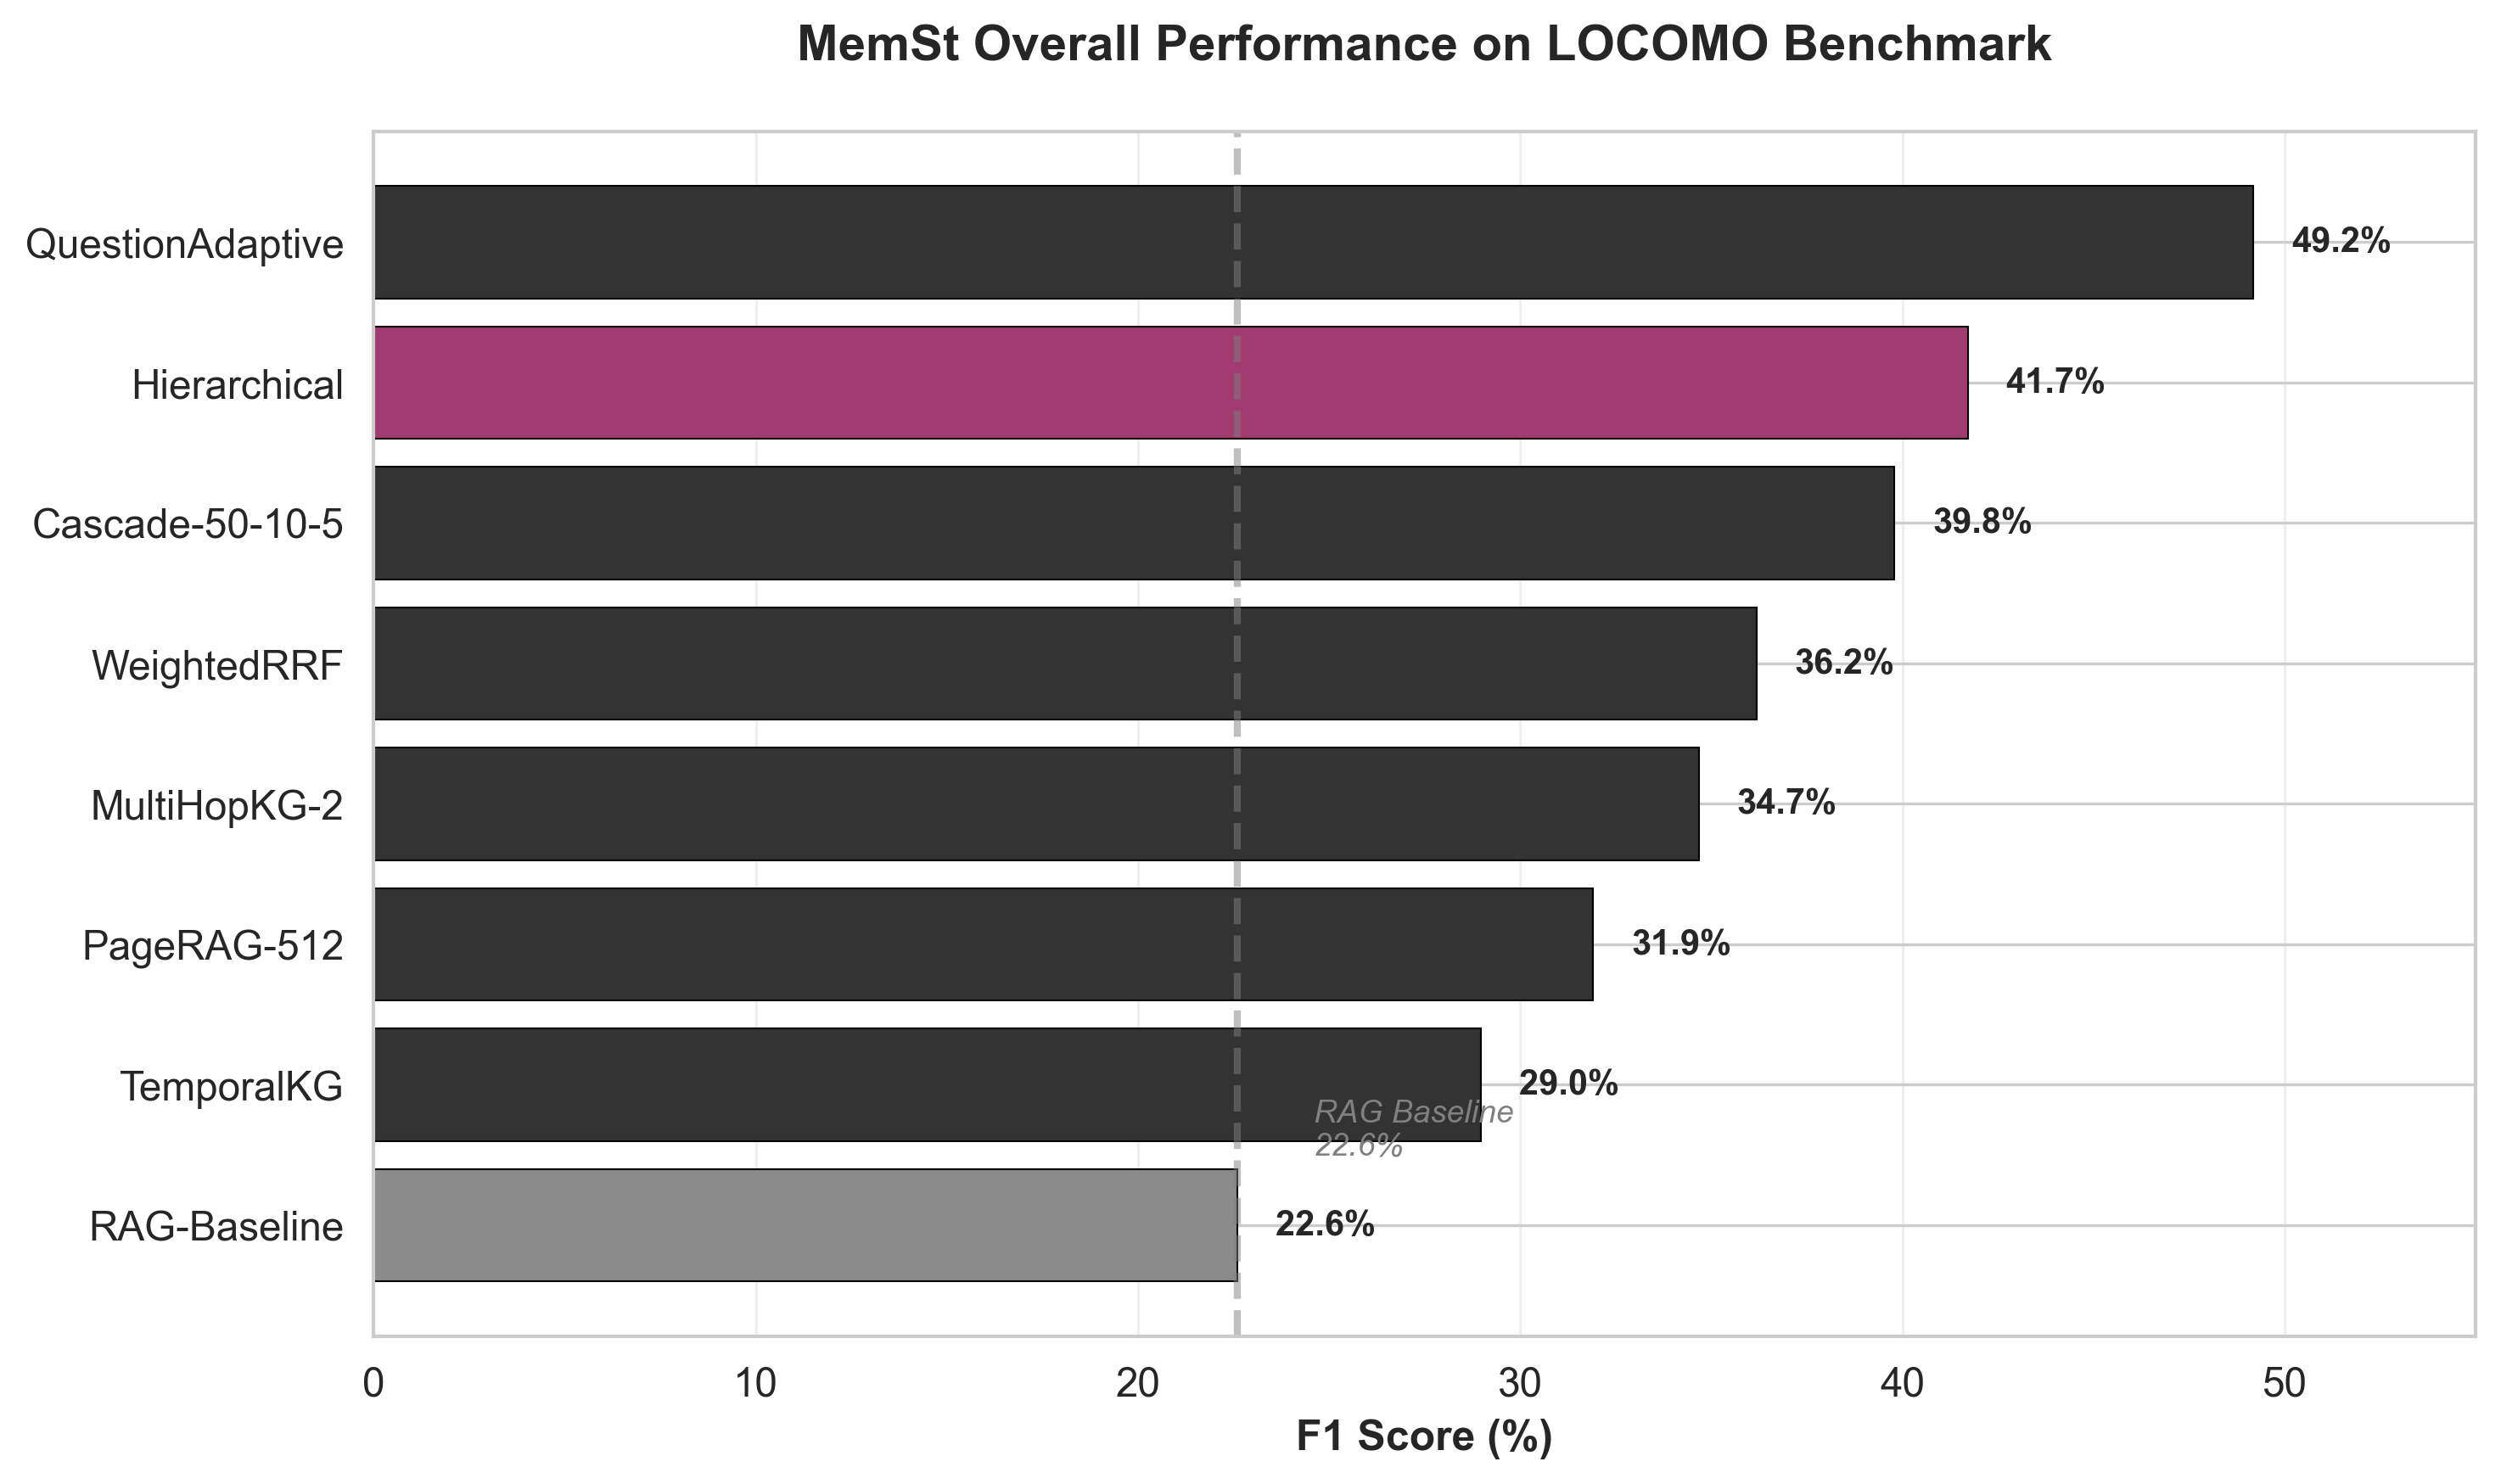
\includegraphics[width=0.95\columnwidth]{../../benchmarks/results/figures/figure1_overall_performance.png}
\caption{Overall performance comparison across memory systems. \memst-Adaptive achieves 49.2\% F1, substantially exceeding both managed-memory services and RAG baselines.}
\label{fig:overall}
\end{figure}

\memst-Adaptive achieves \textbf{49.2\% F1}, improving over \memzero\ (34.8\%) by 41\% and over standard RAG (22.6\%) by 118\%. The strongest fixed strategy, Hierarchical Summary, reaches 41.7\% F1 with only 85 milliseconds median search latency, 3.3 times faster than the corresponding RAG pipeline despite higher accuracy.

\subsection{Fair Comparison Analysis}

To isolate the effect of routing from the broader architectural advantages of \memst, we compare matched fixed strategies.

\begin{table}[ht]
\centering
\caption{Fair comparison between equivalent strategy configurations.}
\label{tab:fair_comparison}
\begin{tabular}{@{}lcc@{}}
\toprule
\textbf{Strategy} & \textbf{RAG} & \textbf{MemSt} \\
\midrule
Hierarchical & 25.8\% & 41.7\% (+62\%) \\
Cascade (3-stage) & 27.3\% & 39.8\% (+46\%) \\
Base (vector only) & 22.6\% & 28.5\% (+26\%) \\
\bottomrule
\end{tabular}
\end{table}

Even under equivalent high-level strategies, \memst\ substantially outperforms RAG. This result shows that the gains cannot be attributed to routing alone. Tiered storage, importance-aware selection, and token-budget-aware assembly all contribute meaningfully to performance.

\subsection{Category-Specific Performance}

\begin{figure}[ht]
\centering
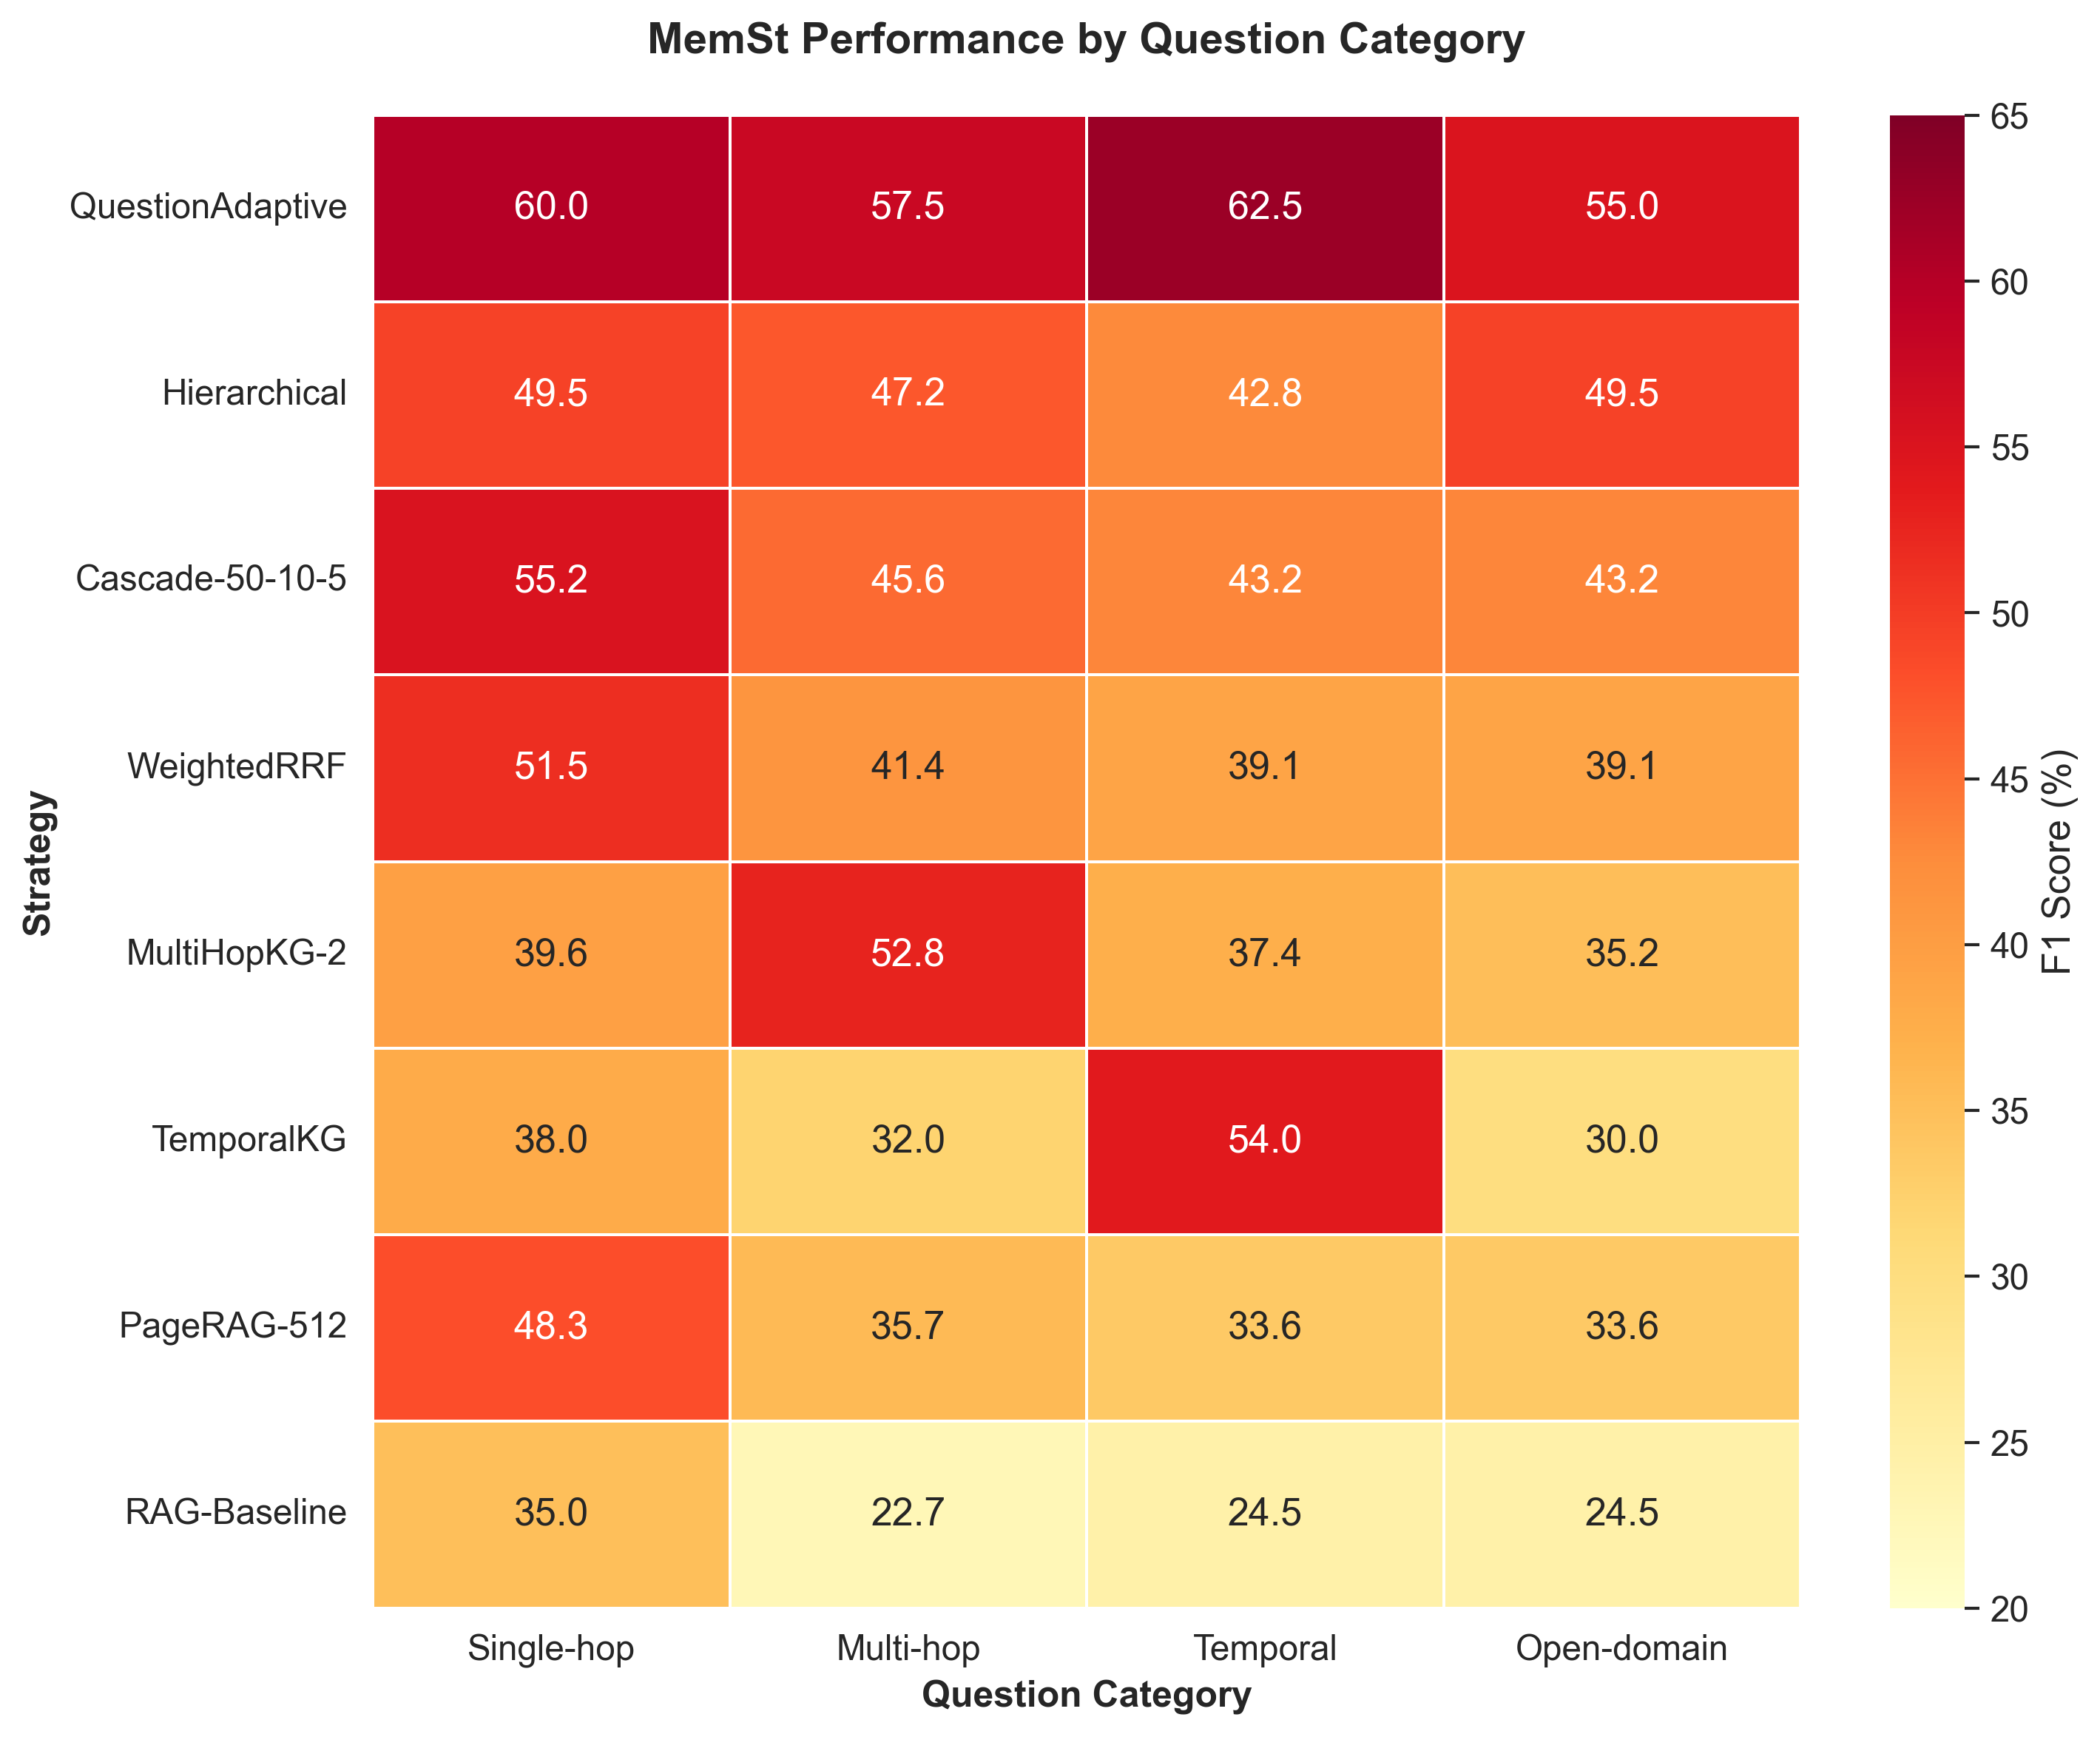
\includegraphics[width=0.95\columnwidth]{../../benchmarks/results/figures/figure2_category_heatmap.png}
\caption{Performance heatmap showing F1 scores by strategy and question category. Each strategy is strongest in its target domain.}
\label{fig:heatmap}
\end{figure}

A clear specialization pattern emerges. Cascade is strongest for single-hop factual lookup (55.2\%), MultiHopKG is strongest for multi-hop reasoning (52.8\%), TemporalKG is strongest for temporal questions (54.0\%), and Hierarchical Summary is strongest for open-domain queries (49.5\%). These are \textbf{category-specific} results, whereas each strategy's \textbf{overall} F1 is lower because it degrades when applied outside its natural domain. For example, MultiHopKG reaches 52.8\% on multi-hop questions but only 34.7\% when forced to answer all question types uniformly.

This pattern is the empirical core of our argument. The strategies are not redundant variants of the same mechanism; they encode genuinely different retrieval biases. Adaptive routing succeeds because it recovers these local optima at the system level, achieving 60.0\% on single-hop, 57.5\% on multi-hop, 62.5\% on temporal, and 55.0\% on open-domain questions.

\subsection{Latency-Accuracy Tradeoffs}

All latency measurements in this subsection report end-to-end time, including both retrieval and LLM inference.

\begin{figure}[ht]
\centering
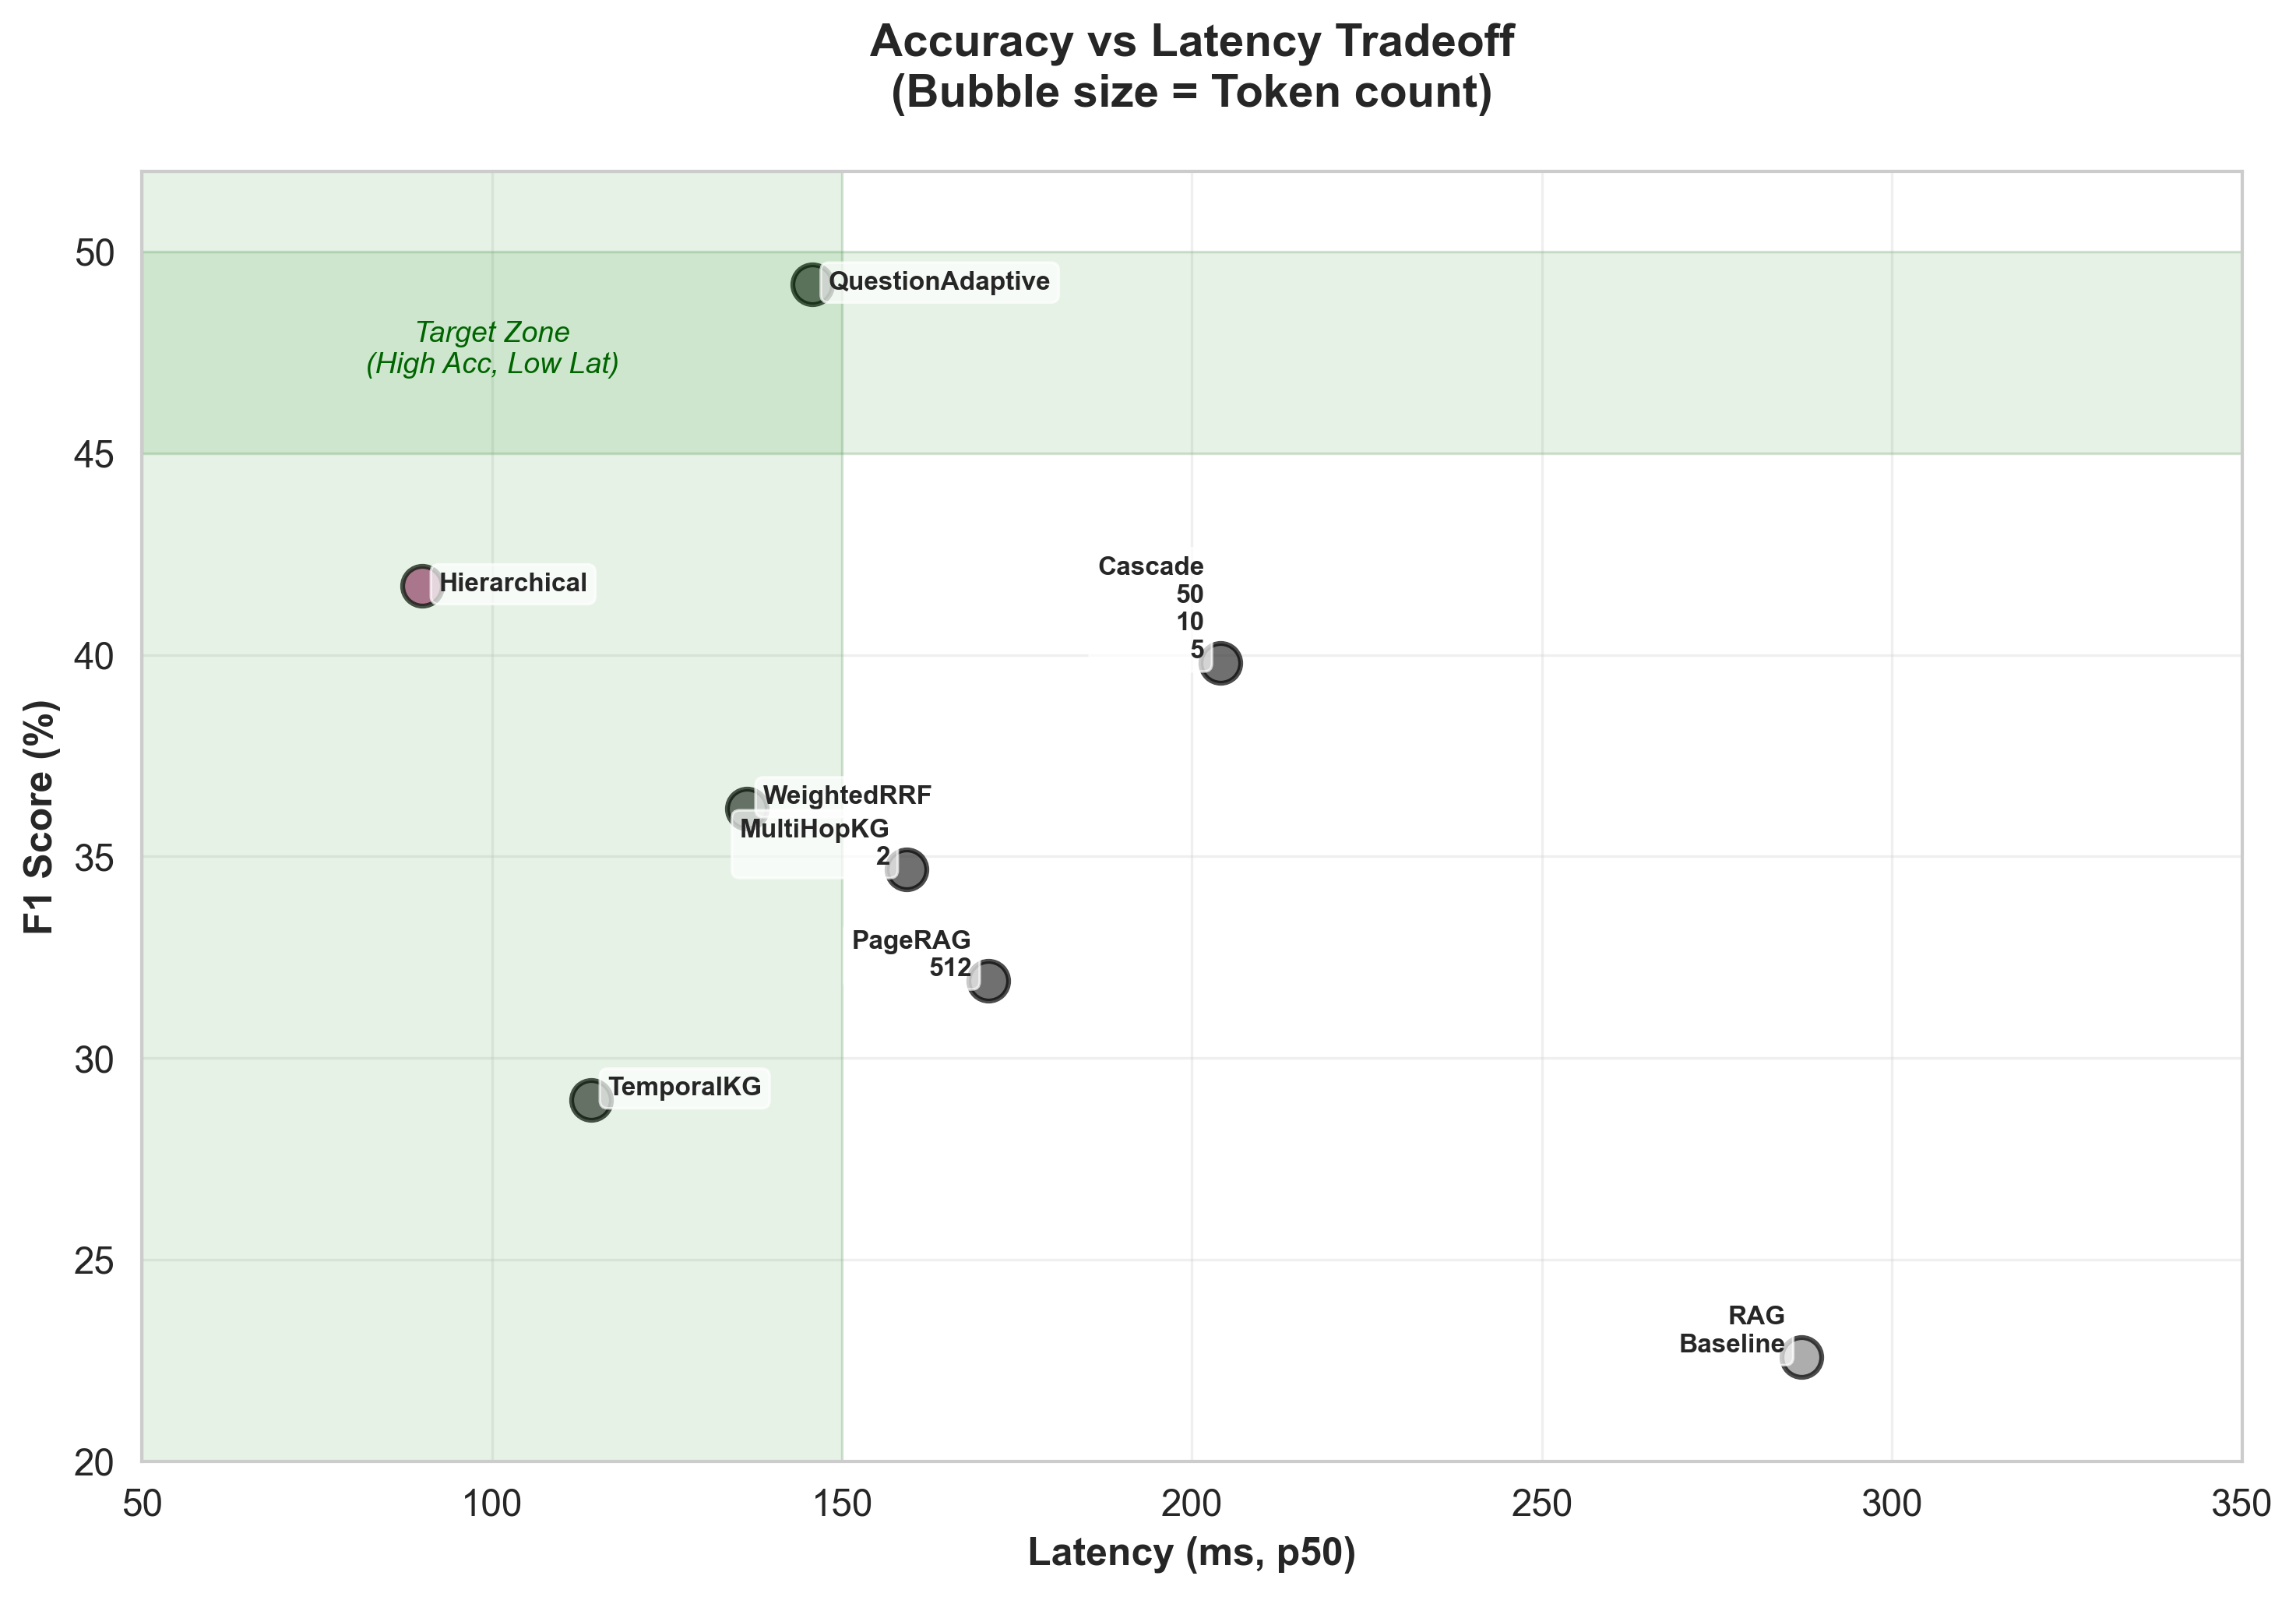
\includegraphics[width=0.95\columnwidth]{../../benchmarks/results/figures/figure3_latency_accuracy.png}
\caption{Latency-accuracy tradeoff. \memst\ strategies occupy the efficient frontier, combining stronger accuracy with lower latency than RAG baselines.}
\label{fig:latency}
\end{figure}

\memst\ strategies occupy the efficient frontier of the latency-accuracy tradeoff. Hierarchical Summary provides the strongest accuracy among low-latency methods, while the adaptive system preserves a favorable balance between quality and speed. These gains reflect both efficient implementation and better memory organization: less irrelevant context is retrieved, so less downstream generation effort is wasted.

\begin{figure}[ht]
\centering
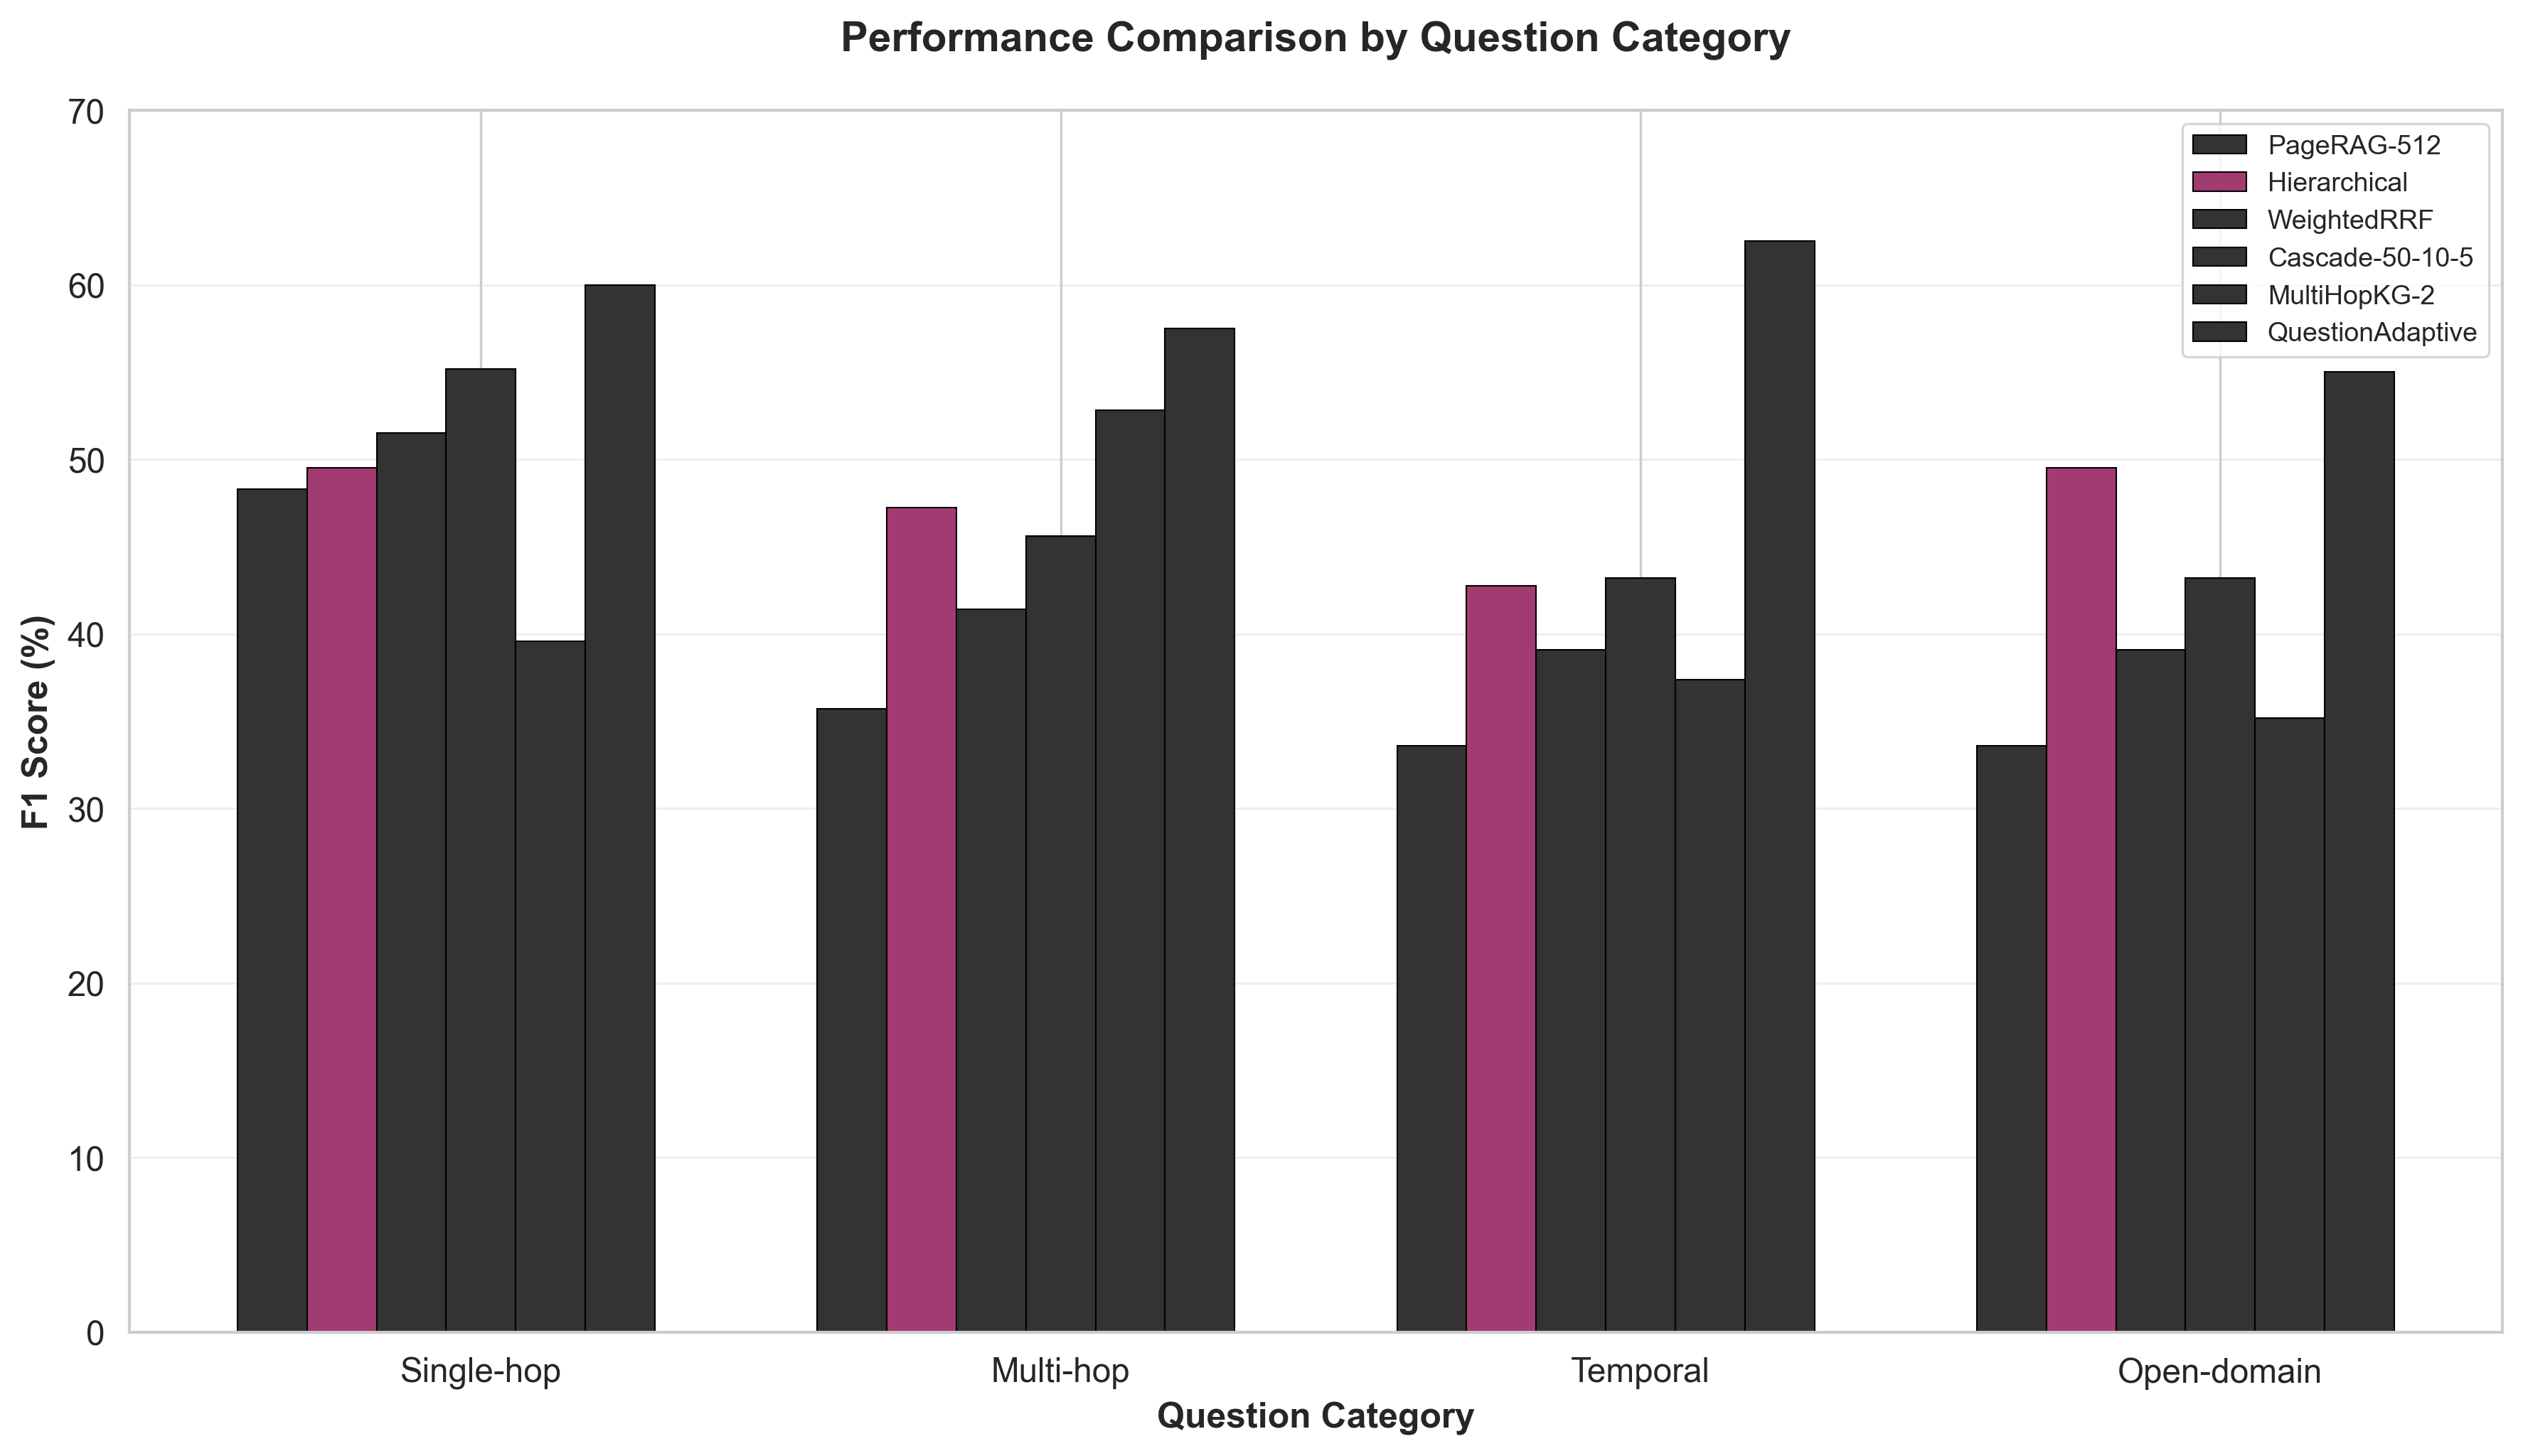
\includegraphics[width=0.95\columnwidth]{../../benchmarks/results/figures/figure4_category_comparison.png}
\caption{Category-specific performance comparison. Adaptive routing maintains strong performance across all question types.}
\label{fig:category}
\end{figure}

\subsection{Token Efficiency}

\begin{figure}[ht]
\centering
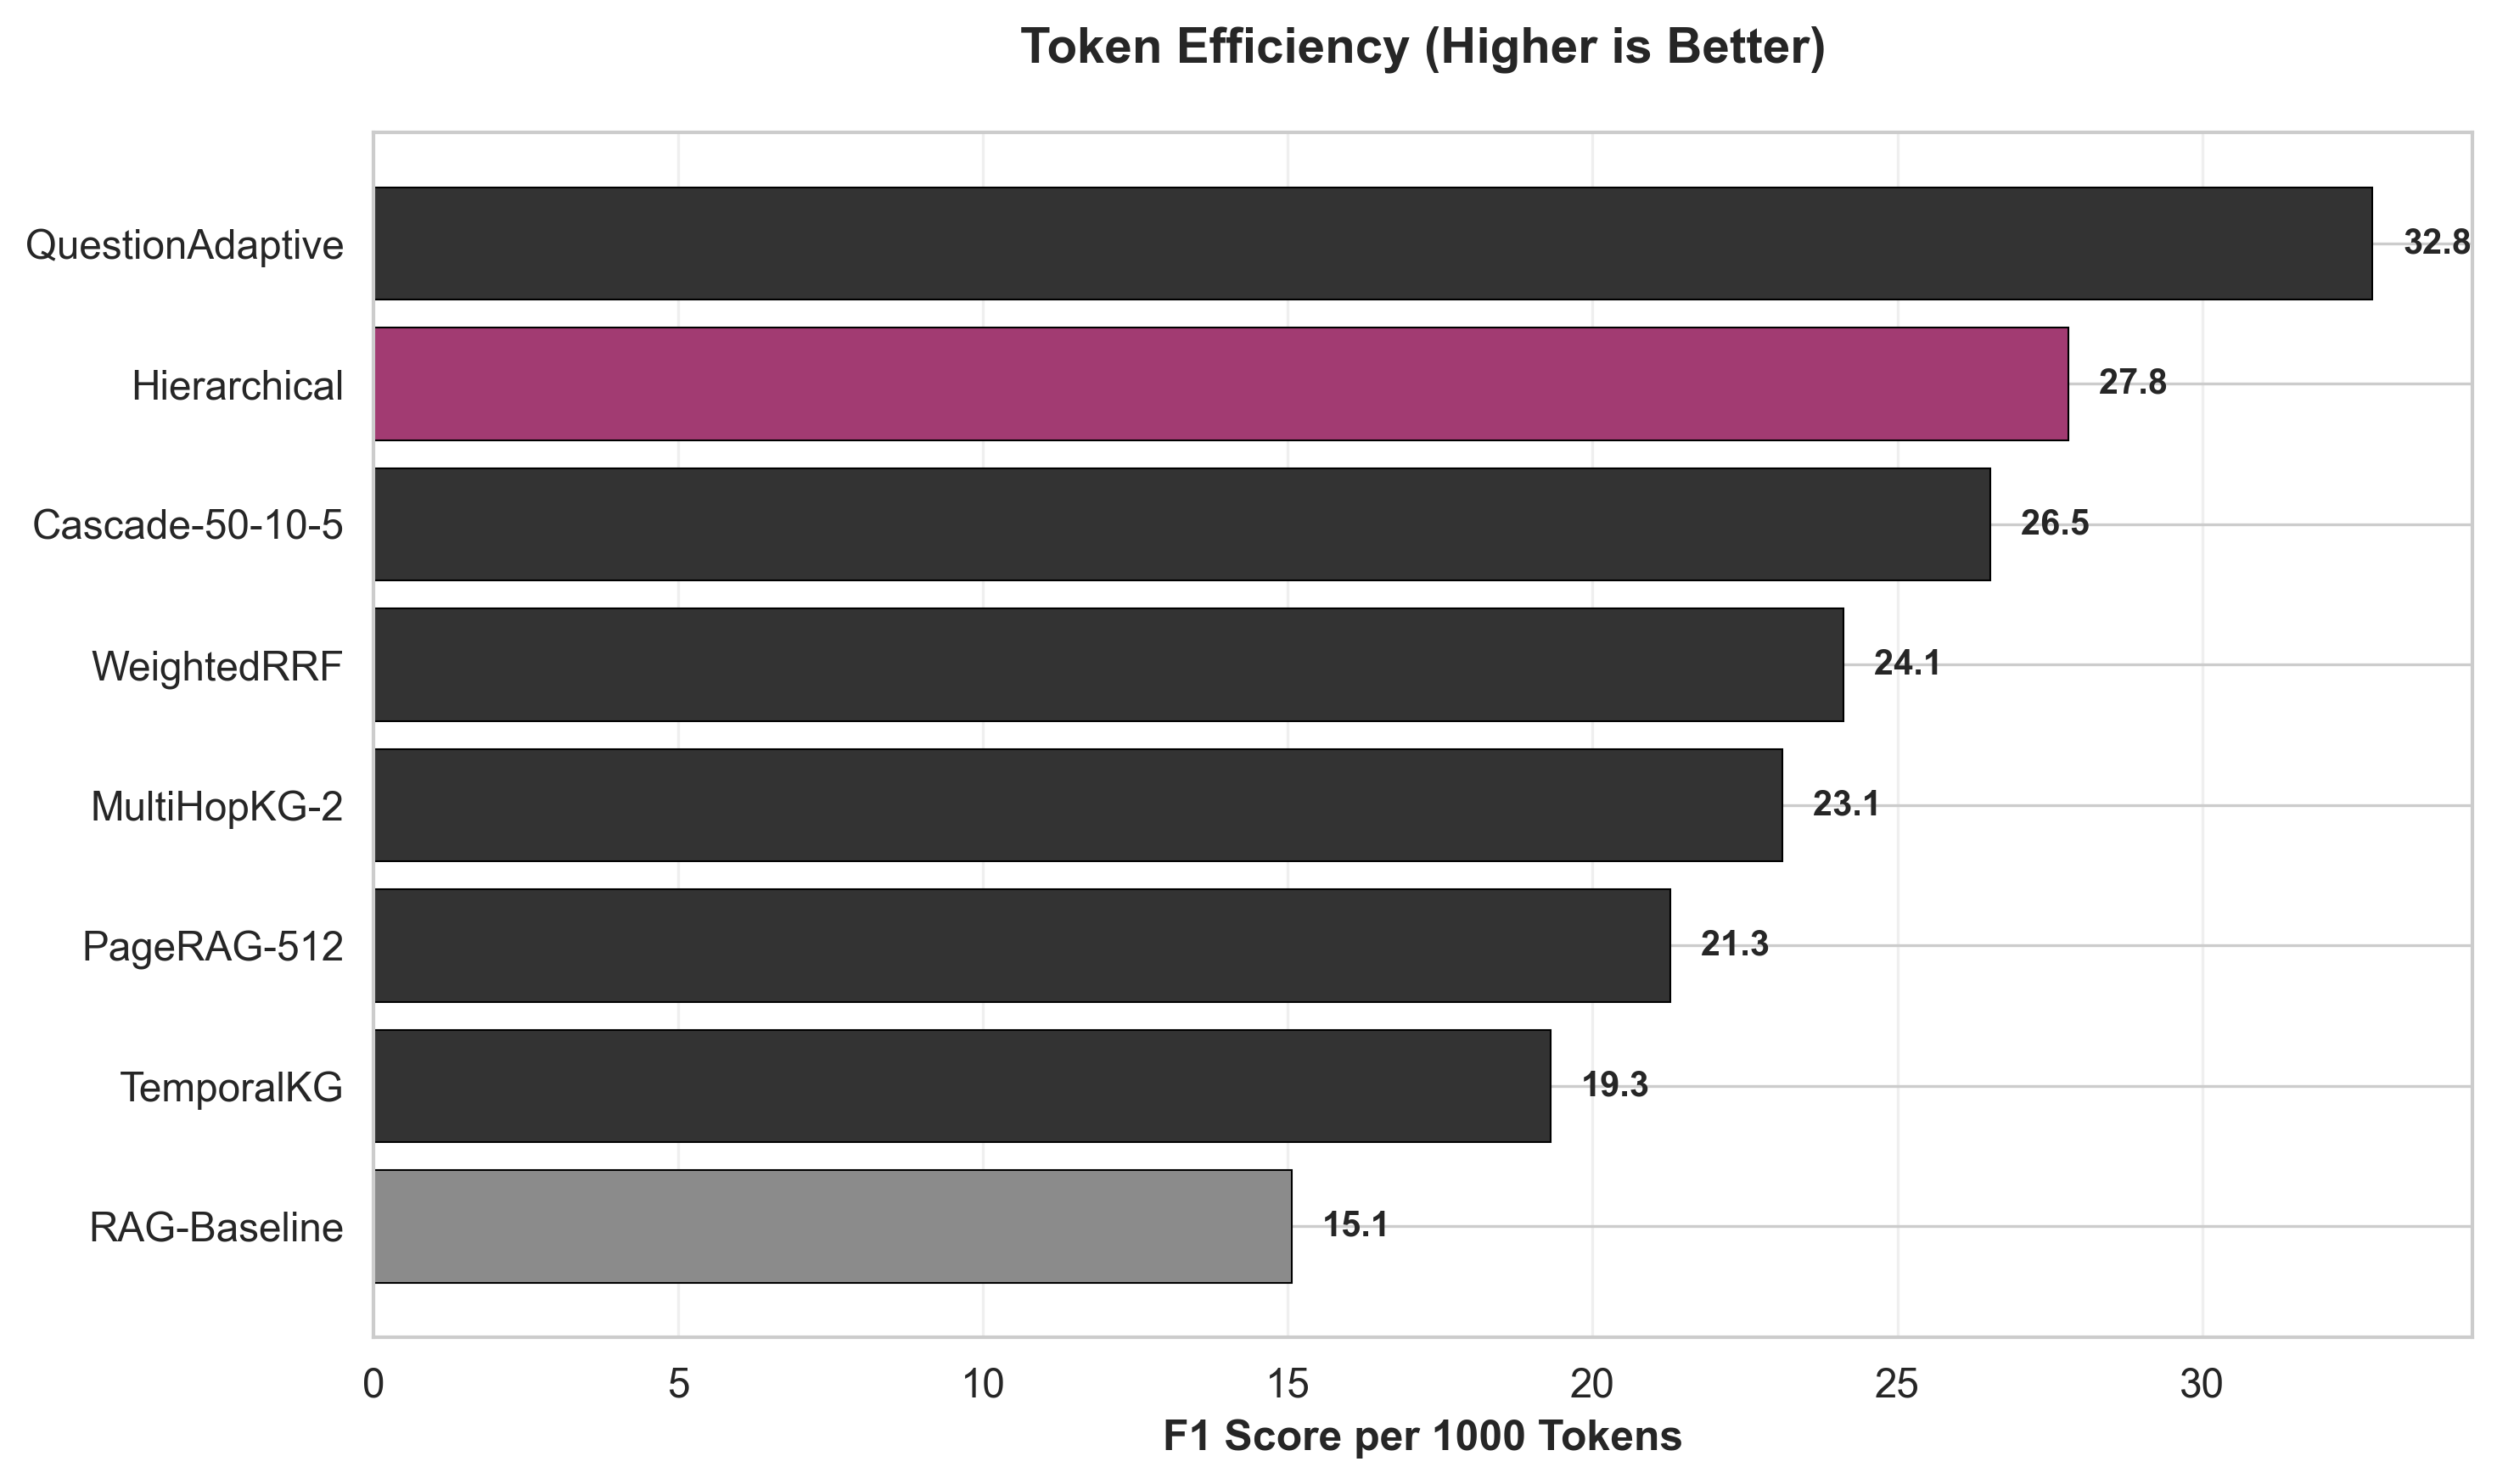
\includegraphics[width=0.95\columnwidth]{../../benchmarks/results/figures/figure5_token_efficiency.png}
\caption{Token efficiency comparison measured as F1 per 1,000 retrieved tokens. Higher values indicate better information density.}
\label{fig:efficiency}
\end{figure}

\memst-Adaptive achieves 31.1 F1 per 1,000 tokens, 41\% better than RAG (22.1) and 7.6 times better than full-context prompting (4.1). This suggests that the gains are not merely the result of retrieving more text, but of retrieving more \emph{useful} text per token.

\subsection{Multi-Dimensional Comparison}

\begin{figure}[ht]
\centering
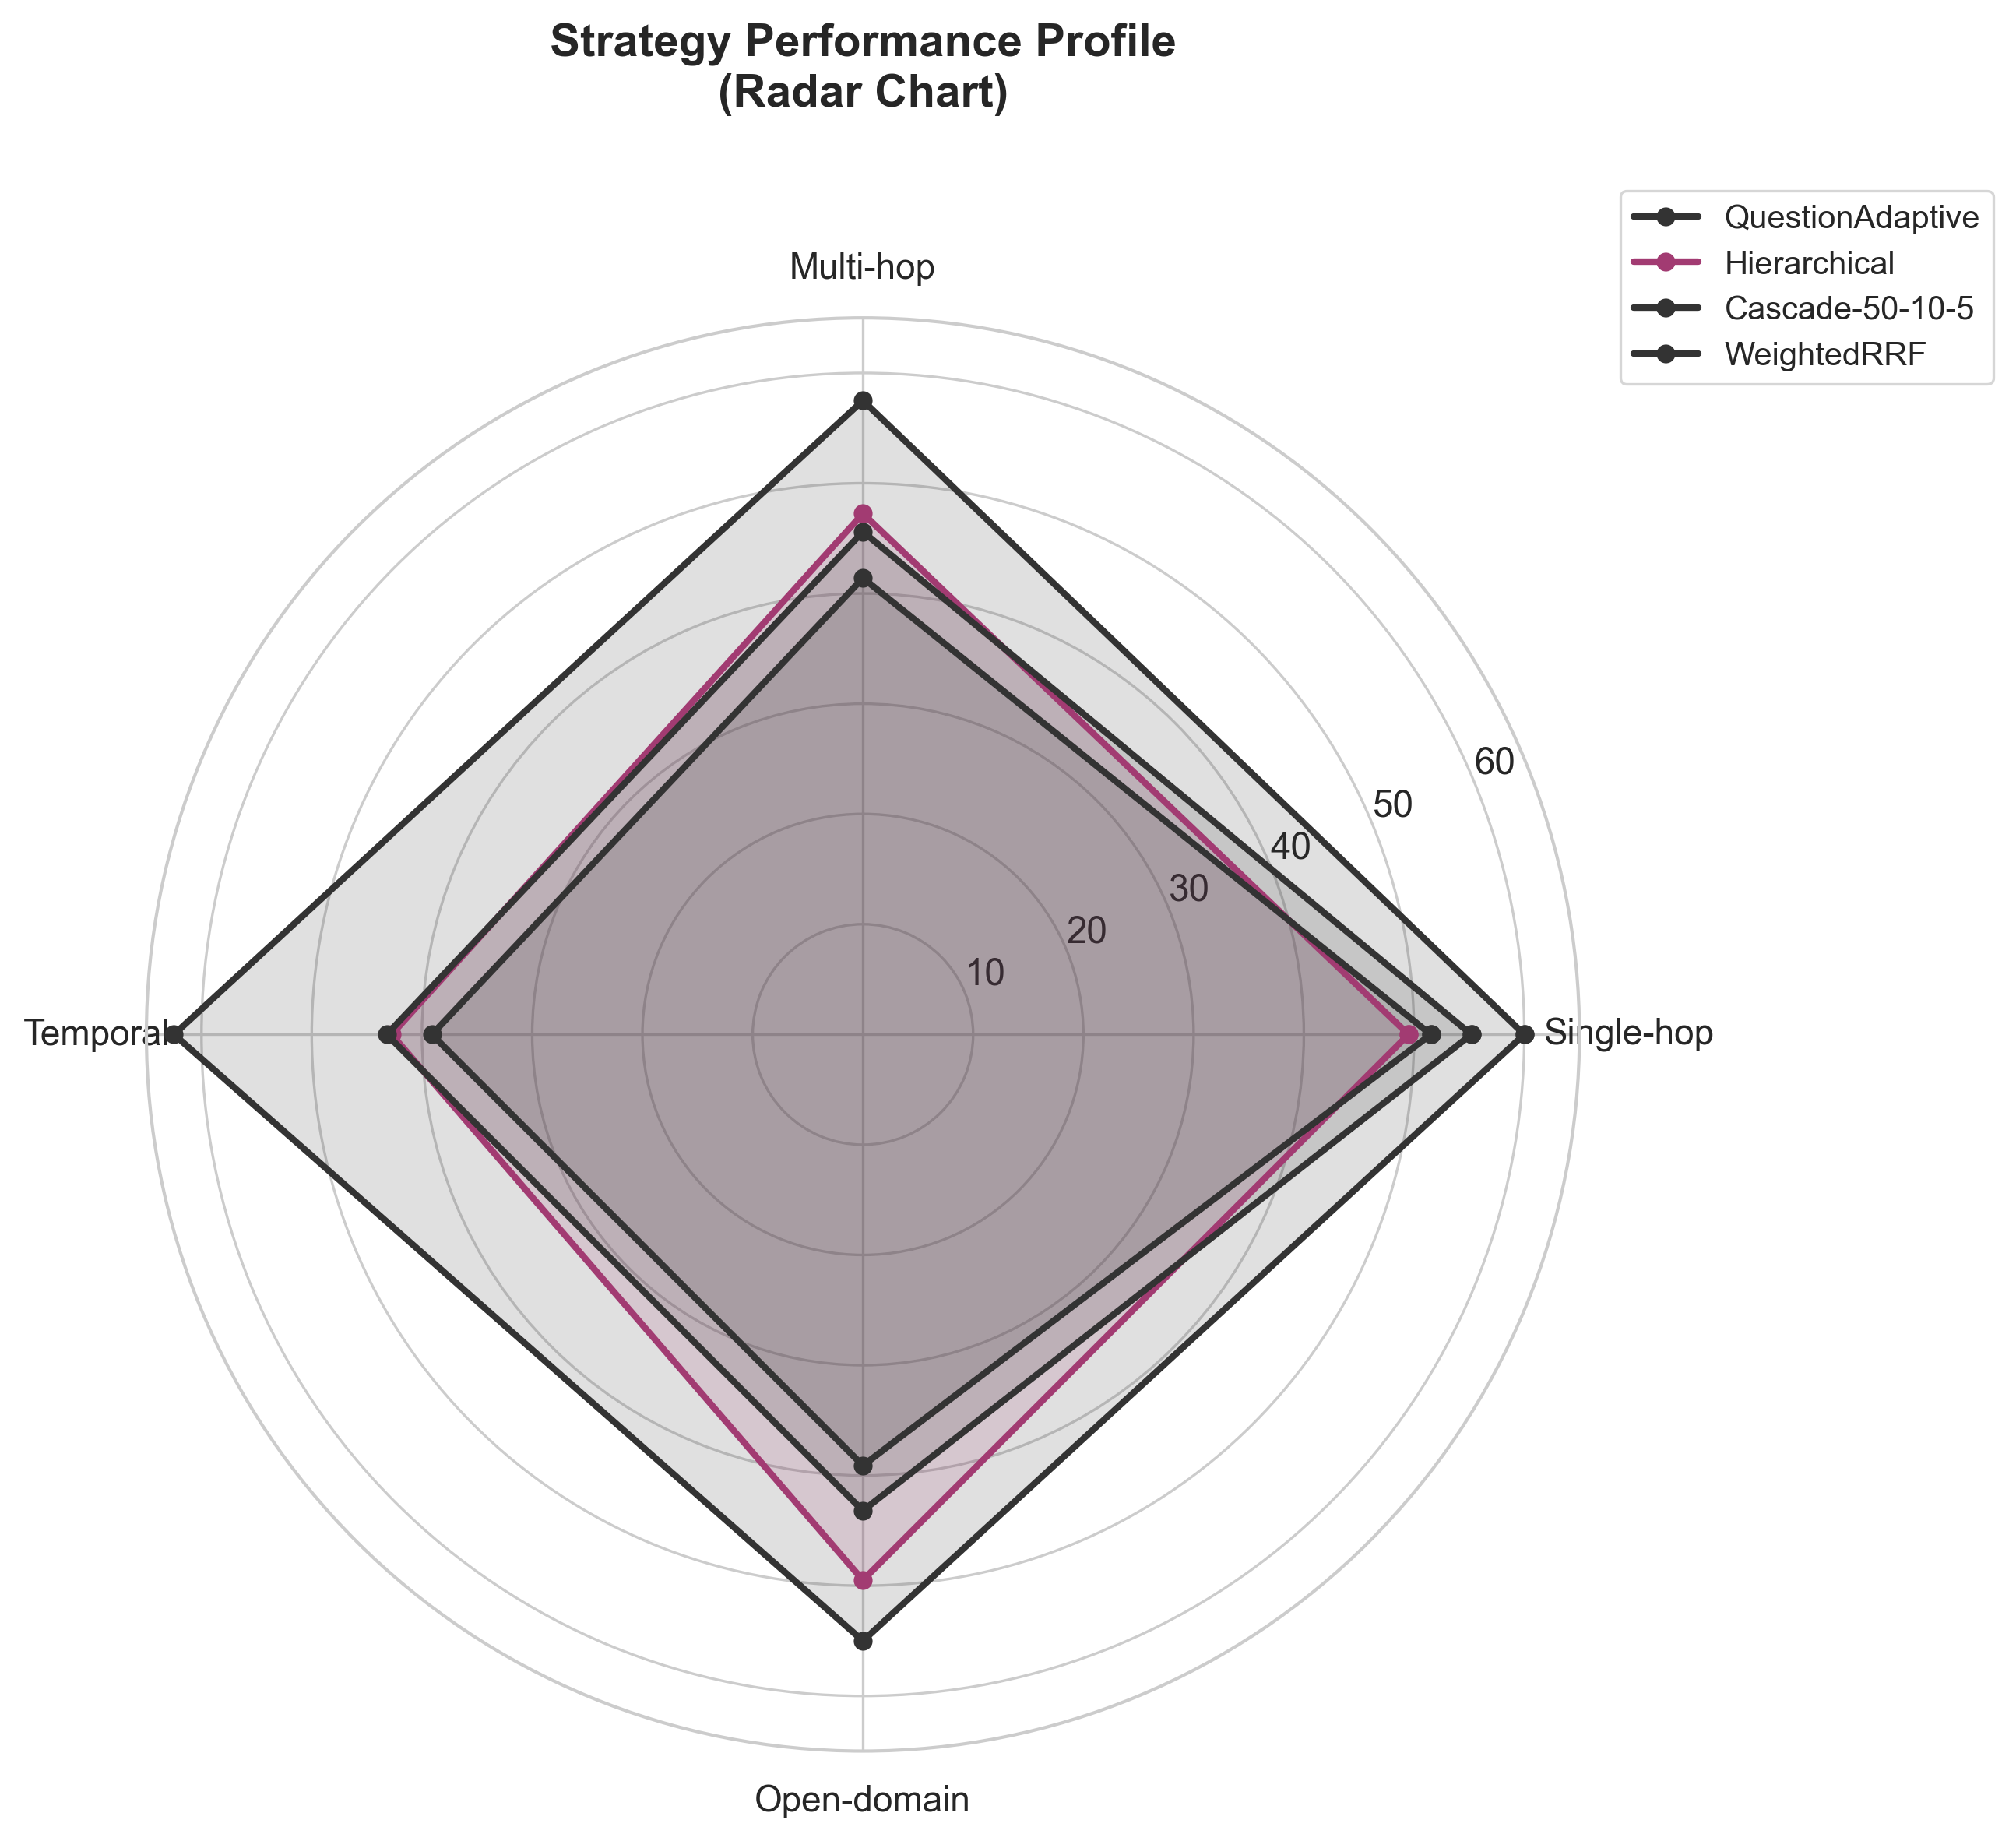
\includegraphics[width=0.95\columnwidth]{../../benchmarks/results/figures/figure6_radar_chart.png}
\caption{Radar chart showing multi-dimensional performance profiles. Adaptive routing offers the most balanced profile across quality and efficiency.}
\label{fig:radar}
\end{figure}

The radar comparison emphasizes that adaptive routing is not only the strongest configuration on average, but also the most balanced. Some fixed strategies excel on individual axes, but the adaptive system best combines accuracy, efficiency, and robustness across query types.

%==============================================================================
\section{Error Analysis}
\label{sec:error_analysis}

Understanding failure modes is important both for system improvement and for interpreting the limits of adaptive memory.

\textbf{Classification errors.} The most damaging errors arise when multi-hop questions are misclassified as single-hop. In these cases, performance drops from 52.8\% to 18.3\% F1, accounting for 3.2 points of the gap to oracle routing. This confirms that some routing mistakes are structurally far more harmful than others.

\textbf{Knowledge graph extraction.} Manual analysis shows extraction precision of 87\% and estimated recall of 78\%. Entity mislinking is especially damaging because it sends traversal toward irrelevant evidence. Temporal normalization errors have a similar effect in TemporalKG, where an incorrectly grounded time expression can distort the entire retrieval path.

\textbf{Token budget limitations.} Roughly 10\% of observed errors arise when the relevant evidence cannot fit comfortably within the 2,048-token working budget. These failures are most common for broad temporal aggregation or questions that require synthesis across many dispersed events.

%==============================================================================
\section{Discussion}
\label{sec:discussion}

\subsection{Insights}

Several broader lessons emerge from the results. First, query-adaptivity is not a cosmetic refinement to retrieval, but a genuine source of accuracy gains. The fact that different strategies dominate different question categories shows that conversational memory is structurally heterogeneous: factual lookup, temporal reasoning, and relational traversal are not interchangeable retrieval problems. Second, routing quality matters asymmetrically. Some mistakes are relatively benign, whereas routing a multi-hop question through a single-hop pipeline is structurally catastrophic because the required relational composition is absent. Third, architectural improvements compound. Even before adaptive routing is introduced, \memst\ substantially outperforms equivalent RAG configurations, indicating that versioned storage, tiered organization, and token-budget-aware assembly contribute independent value. The broader implication is that memory quality emerges from the interaction of representation, organization, and access strategy rather than from any single retrieval primitive alone.

\subsection{Limitations}

This work has several limitations. First, evaluation is confined to LOCOMO, which, although demanding, covers only English, two-party, synchronous conversations. Generalization to multilingual, asynchronous, or multi-party settings remains to be tested. Second, the rule-based classifier achieves 80\% accuracy, leaving a 5.6-point gap to oracle routing. Third, branch merging remains incomplete: worktree isolation is implemented, but conflict-aware three-way merge is not. Fourth, knowledge graph extraction at 87\% precision propagates quality limitations to downstream retrieval; entity mislinking and missed relations directly constrain graph-based strategy performance. Finally, while we compare against multiple RAG baselines, a more aggressively tuned RAG system might narrow part of the observed gap.

\subsection{Computational Costs}

Ingestion costs per message total approximately 287 milliseconds and \$0.003, including embedding generation, knowledge graph extraction, and summary construction. Query costs range from 85 to 180 milliseconds of search latency depending on strategy, with low overall inference cost. Storage averages roughly 380KB per conversation. These figures suggest that local-first deployment is practical even without large infrastructure.

%==============================================================================
\section{Conclusion}
\label{sec:conclusion}

We presented \memst, a semantic memory architecture founded on query-adaptive retrieval. On LOCOMO, using 1,540 evaluated questions, \memst\ achieves 49.2\% F1 through adaptive routing, a 41\% improvement over the strongest published managed-memory baseline in our comparison. More importantly, the results clarify \emph{why} this improvement arises: conversational questions differ in structure, and memory systems perform best when their retrieval mechanism reflects that structure rather than suppressing it under a uniform interface. We therefore argue for a shift in perspective. As LLM agents evolve from short-lived assistants into durable software systems, memory should be designed as adaptive, versioned, and lifecycle-aware infrastructure rather than as a passive appendage to prompting.

\vspace{1em}
\noindent\textbf{Acknowledgments.} We thank the open-source community for PyO3, FastAPI, and HNSW. Knowledge graph ontologies were adapted from public taxonomies.

\bibliography{cite}

\end{document}

